\scanpage{58}
% archive sheet number: 57
\diagram{\begin{tikzcd}[ampersand replacement=\&,column sep=tiny,row sep=large]
\&A_{[x_0x_1x_2x_3]}\&\&\&\&\&\&\\
A_{[x_0x_1x_2]}\arrow[ur]\&A_{[x_1x_2x_3]}\arrow[u]\&\deleted{\unsure{A_{[x_2x_3x_n]}}}\&A_{[x_0x_2x_3]}\arrow[ull]\&A_{[x_0x_1x_3]}\arrow[ulll]\&\&\&\\
A_{[x_0x_1]}\arrow[u]\&A_{[x_1x_2]}\arrow[ul]\arrow[u]\&A_{[x_2x_3]}\arrow[ul]\&\deleted{\unsure{A_{[x_1x_3]}}}\&A_{[x_0x_2]}\arrow[ul]\&A_{[x_0x_3]}\arrow[ull]\arrow[ulllll]\&\deleted{\unsure{A_{[x_0x_3]}}}\arrow[ulllll]\&A_{[x_1x_3]}\arrow[ulll]\\
A_{[x_0]}\arrow[u]\&A_{[x_1]}\arrow[ul]\arrow[u]\&A_{[x_2]}\arrow[ul]\arrow[u]\&A_{[x_3]}\arrow[ul]\&\&\&\&
\end{tikzcd}}
\[\deleted{\unsure{A_{[x_1x_3]}}\quad\unsure{A_{[x_1x_3]}}}\]

\[
\overline{A_{[x_0x_2x_3]}}\cap
\frac{\overline{A_{[x_0x_1x_3]}}}{\overline{A_{[x_0,x_3]}}}
\]
\diagram{\begin{tikzcd}[ampersand replacement=\&,column sep=small,row sep=large]
0\&\&\multicolumn{1}{c}{(A_{[x_0x_2x_3]}+A_{[x_0x_1x_3]})}\&\&\\
\&A_{[x_0x_2]}\arrow[ur]\&A_{[x_1,x_3]}\arrow[u]\&A_{[x_0x_2x_3]}\arrow[ul]\&A_{[x_0x_1x_3]}\arrow[ull]\arrow[dd,bend left=45]\\
0\&A_{[x_0x_2]}\arrow[u]\arrow[urr]\&A_{[x_0x_3]}\arrow[ur]\arrow[urr]\&A_{[x_1x_3]}\arrow[ul]\arrow[ur]\&\\
\&\&\&\&\operatorname{Im}A_{[x_0x_2]}+\operatorname{Im}A_{[x_1x_3]}
\end{tikzcd}}
\[A_{[x_0x_2]}\unsure{*|\times}A_{[x_1,x_3]}\times\bigl(A_{[x_0x_2x_3]}\times A_{[x_0x_1x_3]}\bigr)\]
% The two final factors of the preceding row are enclosed in an oval in the scan.
\figure{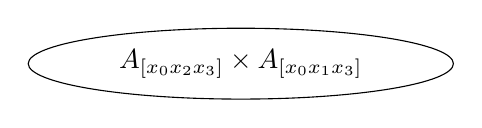
\begin{tikzpicture}\node (a) at (0,0) {$A_{[x_0x_2x_3]}\times A_{[x_0x_1x_3]}$};\draw (0,0) ellipse (2.7 and .45);\end{tikzpicture}}

\diagram{\begin{tikzcd}[ampersand replacement=\&]
\unsure{K_0|S_0}\&S_1\&S_2\&S_{n-1}\&S_n\arrow[l,"d_i^n"]\arrow[d]\\
\&\&\&d_i^n\sigma\&\sigma\\
\&\&\&A_{d_i^n\sigma}\&A_\sigma
\end{tikzcd}}
\[\begin{array}{cccc}\alpha&\beta&-\overline\alpha&-\overline\beta\\\alpha&&0.&\beta\end{array}\]
\noindent\rule{\linewidth}{.3pt}

\[K\qquad d_i^n\qquad0\leq i\leq n+1\qquad d'\pm d''\]
\[
\bigcap_{1\leq i\leq n+1}\operatorname{Ker}d_i^n\qquad
\unsure{\bigcap|\coprod}_{\underline{1\leq i\leq n}}\operatorname{Coker}d_i^n
\]
\[d_i^{n+1}d_0^n x=0\]
si $1\leq i\leq n+2$

\figure{\begin{tikzpicture}[x=.7cm,y=.6cm]
\draw (0,4)--(4,4);\draw[line width=1.4pt] (1.2,4)--(4,4);\foreach \x in {0,1.2,4}{\draw (\x,3.85)--(\x,4.15);}
\draw (-1,3)--(3.5,3);\draw[line width=.8pt] (0,3)..controls (1,2.9) and (2,2.9)..(2.6,3);\foreach \x in {-1,0,2.6,3.5}{\draw (\x,2.85)--(\x,3.15);}
\draw (-4,1)--(-2,1);\draw[line width=1.2pt] (-4,1)--(-2,1);\foreach \x in {-4,-2}{\draw (\x,.85)--(\x,1.15);}
\node[below] at (-3,.8) {$\Delta^n$};
\draw (-1.3,1)--(5,1);\draw[line width=1.2pt] (.6,1)--(2.1,1);\foreach \x in {-1.3,.6,2.1,5}{\draw (\x,.88)--(\x,1.12);}
\node[below] at (.5,.8) {$\Delta^{n+1}$};\node[below] at (4,.8) {$\Delta^{n+2}$};
\draw (-6,-1)--(-5.2,-1);\draw (-4.8,-1)--(-2.3,-1);\foreach \x in {-6,-5.2,-4.8,-2.3}{\draw (\x,-1.1)--(\x,-.9);}
\end{tikzpicture}}
\diagram{\begin{tikzcd}[ampersand replacement=\&]
A_{[x_0,x_2]}\&A_{(x_0,x_0,x_2]}\arrow[l]\\
\&\deleted{\unsure{d}}
\end{tikzcd}}
\[x_0\quad x_1\quad\underbrace{x_{\unsure{i|1}}-x_n}\]
\[\cdot\quad\cdot\quad\cdot\]
$1^\circ)$ $\bigcap$\uline{Ker des dégénérescences}
